\section{Specifying Workflows}\label{specifying-workflows}

Users of cloudmesh cc must follow a certain configuration style to best
specify how a workflow should be run. Customization options include
specifying the job types, the order of how the jobs should be run, and
the portrayal of the graph.

\subsection{Workflow YAML format}\label{workflow-yaml-format}

A workflow yaml file with three Shell script jobs \texttt{a},
\texttt{b}, and \texttt{c} is as follows:

\begin{Shaded}
\begin{Highlighting}[]
\ExtensionTok{workflow:}
  \ExtensionTok{nodes:}
    \ExtensionTok{a:}
       \ExtensionTok{name:}\NormalTok{ a}
       \ExtensionTok{user:}\NormalTok{ gregor}
       \ExtensionTok{host:}\NormalTok{ localhost}
       \ExtensionTok{kind:}\NormalTok{ local}
       \ExtensionTok{status:}\NormalTok{ ready}
       \ExtensionTok{label:} \StringTok{\textquotesingle{}\{name\}\textbackslash{}nprogress=\{progress\}\textquotesingle{}}
       \ExtensionTok{script:}\NormalTok{ test{-}a.sh}
    \ExtensionTok{b:}
       \ExtensionTok{name:}\NormalTok{ b}
       \ExtensionTok{user:}\NormalTok{ gregor}
       \ExtensionTok{host:}\NormalTok{ localhost}
       \ExtensionTok{kind:}\NormalTok{ local}
       \ExtensionTok{status:}\NormalTok{ ready}
       \ExtensionTok{label:} \StringTok{\textquotesingle{}\{name\}\textbackslash{}nprogress=\{progress\}\textquotesingle{}}
       \ExtensionTok{script:}\NormalTok{ test{-}b.sh}
    \ExtensionTok{c:}
      \ExtensionTok{name:}\NormalTok{ c}
      \ExtensionTok{user:}\NormalTok{ gregor}
      \ExtensionTok{host:}\NormalTok{ localhost}
      \ExtensionTok{kind:}\NormalTok{ local}
      \ExtensionTok{status:}\NormalTok{ ready}
      \ExtensionTok{label:} \StringTok{\textquotesingle{}\{name\}\textbackslash{}nprogress=\{progress\}\textquotesingle{}}
      \ExtensionTok{script:}\NormalTok{ test{-}c.sh}
  \ExtensionTok{dependencies:}
    \ExtensionTok{{-}}\NormalTok{ a,b,c}
\end{Highlighting}
\end{Shaded}

\subsection{Example Workflows}\label{example-workflows}

Sample yaml files can be found at the following link:

\url{https://github.com/cloudmesh/cloudmesh-cc/blob/main/tests/workflow-example/workflow-example.yaml}

\subsection{Defining nodes in the
workflow}\label{defining-nodes-in-the-workflow}

Nodes can be customized in various ways within the workflow
configuration YAML file, including their job types (python, sh, jupyter,
or slurm), their virtual Python environment (by specifying
\texttt{venv}), their appearance on the graph, and other
characteristics.

\subsubsection{Defining labels for the
workflow}\label{defining-labels-for-the-workflow}

These variables must be in curly braces when defining the labels inside
the yaml workflow files.

For example, a label could be defined as follows:

\begin{Shaded}
\begin{Highlighting}[]
\NormalTok{workflow:}
\NormalTok{  nodes:}
\NormalTok{    start:}
\NormalTok{      label: \textquotesingle{}start\textbackslash{}nCreated=\{created.\%Y/\%m/\%d, \%H{-}{-}\%M{-}{-}\%S\}\textbackslash{}nWorkflow Started=\{t0.\%Y/\%m/\%d, \%H{-}{-}\%M{-}{-}\%S\}\textbackslash{}nNow=\{now.\%Y/\%m/\%d, \%H{-}{-}\%M{-}{-}\%S\}\textbackslash{}nElapsed=\{dt0.\%M{-}{-}\%S\}\textquotesingle{}}
\end{Highlighting}
\end{Shaded}

This creates a node on the graph that looks similar to the following
example:

\begin{figure}
\centering
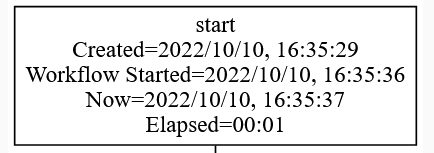
\includegraphics{images/labelmaker-example.png}
\caption{An example node with labels}
\end{figure}

Initially, the created and elapsed labels are \texttt{N/A} if the
workflow has not yet started, but they are replaced during runtime. This
can be observed by running a workflow in graph view in the web
interface.

Colons must be replaced with \texttt{-\/-} and the years, months, days,
hours, minutes, and seconds can be arranged as desired, as long as the
corresponding letters remain consistent (\texttt{\%Y} \texttt{\%m}
\texttt{\%d} \texttt{\%H} \texttt{\%M} \texttt{\%S} respectively). Also,
the format of the time must come immediately following the period.

\begin{itemize}
\tightlist
\item
  \texttt{name} name of job
\item
  \texttt{progress} progress of job from 0-100
\item
  time labels:

  \begin{itemize}
  \tightlist
  \item
    \texttt{now.} current time
  \item
    \texttt{now.\%Y/\%m/\%d,\ \%H-\/-\%M-\/-\%S} now in particular
    format (this can be used for other times as well)
  \item
    \texttt{created.} time when workflow was created
  \item
    \texttt{t0.} workflow start time
  \item
    \texttt{t1.} workflow end time
  \item
    \texttt{dt0.} elapsed time since workflow began
  \item
    \texttt{dt1.} total time of workflow once complete
  \item
    \texttt{tstart.} job start time
  \item
    \texttt{tend.} job end time
  \item
    \texttt{modified.} job modified time
  \end{itemize}
\item
  \texttt{os.} operating system environment variable (like os.HOME)
\item
  \texttt{cm.} cloudmesh variable that is read from \texttt{cms\ set}
\end{itemize}

\subsection{Defining format for timestamp
labels}\label{defining-format-for-timestamp-labels}

Various formats can be used for the timestamps, such as the American
datetime format \texttt{\%m/\%d/\%Y,\ \%H-\/-\%M-\/-\%S} or the
international datetime format \texttt{\%Y/\%m/\%d,\ \%H-\/-\%M-\/-\%S}.
As long as the letters stay consistent (\texttt{\%Y} \texttt{\%m}
\texttt{\%d} \texttt{\%H} \texttt{\%M} \texttt{\%S} for year, month,
day, hour, minute, and second, respectively), any format can be created.

If no format is specified following the period after the variable, the
datetime defaults to American format.

\subsection{Defining graphviz shapes and
styles}\label{defining-graphviz-shapes-and-styles}

Any shape and style for the nodes in the graph can be chosen, as long as
they are taken from the graphviz documentation:

\url{https://graphviz.org/doc/info/shapes.html}

\url{https://graphviz.org/docs/attr-types/style/}

The following is an example of a node in YAML format that uses a box
shape and an empty style. The empty style defaults to \texttt{filled},
which allows the node to change color when the job status is changed.

\begin{Shaded}
\begin{Highlighting}[]
\NormalTok{workflow:}
\NormalTok{  nodes:}
\NormalTok{    start:}
\NormalTok{      label: \textquotesingle{}start\textbackslash{}nCreated=\{created.\%Y/\%m/\%d, \%H{-}{-}\%M{-}{-}\%S\}\textbackslash{}nWorkflow Started=\{t0.\}\textbackslash{}nElapsed=\{dt0.\}\textquotesingle{}}
\NormalTok{      kind: local}
\NormalTok{      user: grey}
\NormalTok{      host: local}
\NormalTok{      status: ready}
\NormalTok{      exec: \textquotesingle{}echo hello\textquotesingle{}}
\NormalTok{      name: start}
\NormalTok{      shape: box}
\NormalTok{      style: \textquotesingle{}\textquotesingle{}}
\end{Highlighting}
\end{Shaded}

\subsection{Defining dependencies in the
workflow}\label{defining-dependencies-in-the-workflow}

Dependencies are specified in the order which jobs should be run, from
left to right. They are listed under the workflow in the yaml file.

\begin{Shaded}
\begin{Highlighting}[]
\ExtensionTok{workflow:}
  \ExtensionTok{nodes:}
    \ExtensionTok{a:}
       \ExtensionTok{name:}\NormalTok{ a}
    \ExtensionTok{b:}
       \ExtensionTok{name:}\NormalTok{ b}
    \ExtensionTok{c:}
       \ExtensionTok{name:}\NormalTok{ c}
  \ExtensionTok{dependencies:}
    \ExtensionTok{{-}}\NormalTok{ a,b,c}
\end{Highlighting}
\end{Shaded}

\subsection{Reporting Progress}\label{reporting-progress}

When running scripts/jobs inside a workflow, the scripts must leverage
some format of cloudmesh.progress to run successfully. Otherwise, the
Workflow class cannot tell if the scripts are done, breaking the
progress functionality.

The examples that are provided with cloudmesh-cc are already augmented
with cloudmesh.progress. Thus, if a user is running self-made jobs and
workflows, they must adhere to the guidelines as follows.

\subsection{Shell and Slurm Scripts}\label{shell-and-slurm-scripts}

For shell and Slurm scripts \texttt{.sh}, the script must contain:

\begin{Shaded}
\begin{Highlighting}[]
\BuiltInTok{echo} \StringTok{"\# cloudmesh status=running progress=1 pid=}\VariableTok{$$}\StringTok{"}
\end{Highlighting}
\end{Shaded}

at the beginning of the script, and

\begin{Shaded}
\begin{Highlighting}[]
\BuiltInTok{echo} \StringTok{"\# cloudmesh status=done progress=100 pid=}\VariableTok{$$}\StringTok{"}
\end{Highlighting}
\end{Shaded}

at the end of the script.

\subsection{Python Scripts and Jupyter
Notebooks}\label{python-scripts-and-jupyter-notebooks}

For Python scripts \texttt{.py} and Jupyter notebooks \texttt{.ipynb},
the script must contain an import module from cloudmesh.common and calls
to the progress function.

py\_script.py

\begin{Shaded}
\begin{Highlighting}[]
\ExtensionTok{from}\NormalTok{ cloudmesh.common.StopWatch import progress}
\ExtensionTok{from}\NormalTok{ cloudmesh.common.Shell import Shell}
\ExtensionTok{filename}\NormalTok{ = Shell.map\_filename}\ErrorTok{(}\StringTok{\textquotesingle{}./py\_script.log\textquotesingle{}}\KeywordTok{)}\ExtensionTok{.path}
\ExtensionTok{progress}\ErrorTok{(}\VariableTok{progress}\OperatorTok{=}\NormalTok{1, }\VariableTok{filename}\OperatorTok{=}\NormalTok{filename}\KeywordTok{)}

\CommentTok{\# your script does what you want it to do here...}

\ExtensionTok{progress}\ErrorTok{(}\VariableTok{progress}\OperatorTok{=}\NormalTok{100, }\VariableTok{filename}\OperatorTok{=}\NormalTok{filename}\KeywordTok{)}
\end{Highlighting}
\end{Shaded}

The statements do not need to be at the absolute beginning or end of the
script, but the progress must:

\begin{itemize}
\tightlist
\item
  be written to a filename with the same name as the script, ending in
  \texttt{.log}
\item
  begin at progress=1
\item
  and end at progress=100
\end{itemize}
